\documentclass[english]{report}
\usepackage[letterpaper,left=1in,top=1in,right=1in,bottom=1in,portrait,twoside=true, headheight=110pt]{geometry}
\usepackage{graphicx}
\usepackage{color}
\usepackage{fancyhdr}
\pagestyle{fancy}

\renewcommand{\chaptermark}[1]{\markright{#1}{}}
\renewcommand{\sectionmark}[1]{\markright{#1}{}}
\usepackage{amsmath}
\usepackage{framed}



\rhead{ID: 804057531 Christian Gao}


\usepackage{Sweave}
\begin{document}
\Sconcordance{concordance:MV_report.tex:MV_report.Rnw:%
1 17 1 1 0 2 1 1 199 56 1 1 3 1 2 9 1 1 5 1 2 1 5 1 2 1 5 1 2 7 1 4 2 1 %
1 6 2 18 1}



\begin{center}\bf\Large
New Modern Portfolio Theory\\ \normalfont
Christian Gao
\end{center}
\tableofcontents
\newpage


\section{Intro}

\Large{Previous studies in portfolio theory have shown that by diversifying portfolios with a variety of financial assets, one can successfully reduce the risk of investments while still preserving the return of the portfolio. This concept, although illustrated in the current Mean Variance (MV) Model, is presented with three major flaws due to the difficulty in designing a structure that can closely fit reality. First, the current MV model does not take into account that past returns are not as influential as current returns. Second, the Mean Variance model heavily favors high volatility securities. Finally, the Mean Variance Model describes the overall volitility of the stock but does not accurately describe risk. Our new model is based on the school of thought that risk is defined by the size of the errors between our predicted value and the actual value rather than the standard deviation of returns. So risk depends on the quality of the model not just the movement of the stock. To suggest a more unbiased way of estimating the true mean variance curve we set three assumptions about our data.
}

\Large{\bf New Assumptions for the New MV model}

\begin{enumerate}
  \item Samples ordered according to time.
  \item Newer events affect predictions more than older events and its effect decays exponentially.
  \item Future Predictions are comprised of a point estimate and Trend component.
\end{enumerate}

\newpage
\section{Flaws of Old MV Model}

\subsection{Mean Return Does not Equal Expected Return}

\Large{The greatest flaw in the old mean variance model is its tendency to favor volitile stocks over non-volitile stocks. Consider the equation for returns.}\\

\LARGE{\(\frac{P_{t=2}-P_{t=1}}{P_{t=1}}\)}\\

\Large{Suppose a stock went from two dollars to one dollar then back to two dollars. According to this equation, we would loose 50\% then gain 100\% even though we have not accumulated any real gains. This is very problematic as this makes the Mean Variance model very biased when applied to volitile stocks. Since we are essentially inventing returns with this model, the model will almost always show an upper bound curve because more volitile stocks are mathematically guaranteed to have a higher return. Supposed we instead took a weighted return so that denominator is the same for the two calculations.}

\LARGE{\(\frac{P_{t=2}-P_{t=1}}{Mean(P_{t=1},P_{t=2})}\)}\\

\Large{Then in the previous example we would first loose 66\% then gain 66\%. At first glance this seems good, however, since we are using one number to generalize the returns of a stock, we are making the assumption that the stock is exponentially destributed. Suppose we have a stock that started at one dollar and ended up at twenty dollars. It the stock grew by one dollar every year, the first few years will see very high growth such as from one dollar to two dollars but the last few years the percentage returns will decay. If we simply take the average of the returns then in the coming years then this will highly overestimate the expected return of the stock which may show a trend of growth that is slowing down. In other words this way of calculating returns gives the most optimistic assumption that the stock has an exponential trend, and this estimate will be biased if the real trend of the stock is for example linear. }

\subsection{Variance in Returns Does not Equal Risk}

\Large{The second flaw in the MV model is the estimation of risk. Supposed stock one went up in price exactly one percent every day for the past ten days, the model would classify that as no risk because there is no difference between the average percentage of increase and the actual percentage of increase every day. Suppose stock two went up in price of one dollar every day. Then the model would return a risk bigger than 0 because even though the collar returns are constant the percentage returns change over time. Thus, stocks with a linear trend are seen as higher risk than stocks with an exponential trend. This means that the MV model cannot capture any pattern or trend that is not exponential and will always assume that a stock growing exponentially is the least volitile stock.  }

\newpage
\section{New MV Model- Intro to Exponential Smoothing}

\subsection{Basic Double Exponential Smoothing}

\Large{In this section we will propose a model that will help solve the biased nature of the old MV model. For the base of our new MV model we will use the Holt-Winters double exponential. The model is suitable for our needs because its parameters illustrates one of our new assumptions. The new "mean" or expected return will be defined as the predicted value of the next time period or periods into the future. The new variance will be defined as the difference between our previous predictions as the actual value. The Holt-Winters smoother separates each new predicted value into two characteristics a trend and a point estimate. The smoothed value \( s_t \)is a weighted average between the current stock price and the previous trend and smoothed stock estimate. The trend \( b_t \) is the current direction that the stock is currently moving in and is a exponentially decaying average of all the pervious movements in time. Alpha and Beta describe how much we value current data vs old data. The closer they are to 0 the more we value old data.}\\

\noindent
\Large{
\( s_1 = x_1 \)\\
\( b_1 = x_1 - x_0 \) \\
\( s_t = \alpha x_t + (1-\alpha )(s_{t-1} + b_{t-1}) \) \\
\( b_t = \beta(s_t - s{t-1}) + (1-\beta)b{t-1} \) \\
\( F_{t+m} = s_t + mb_t \)
}

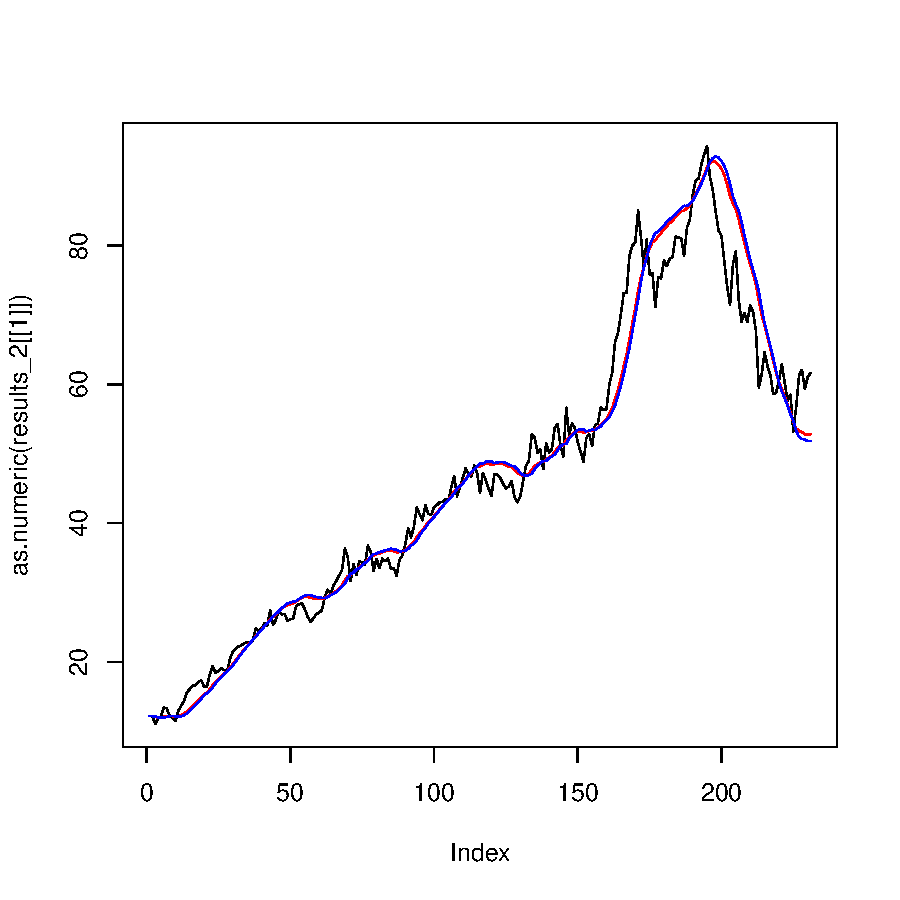
\includegraphics{MV_report-002}

\newpage
\subsection{Exponential Smoothing with added Greed Variable}

\Large{
\( F_{t+m} = s_t + mb_t \)\\
\( F_{t+m} = G(x_t) + (1-G)s_t + mb_t \)}

\Large{Here I have added a greed constant to the prediction equation. When G is zero, it is the normal prediction model that predicts the next value based on the smoothed estimate and the current trend. Then G is one we attach the trend to the current stock price instead of the smoothed value allowing us to make better predictions for the near future. The lower G is the more into the future you want to predict.}

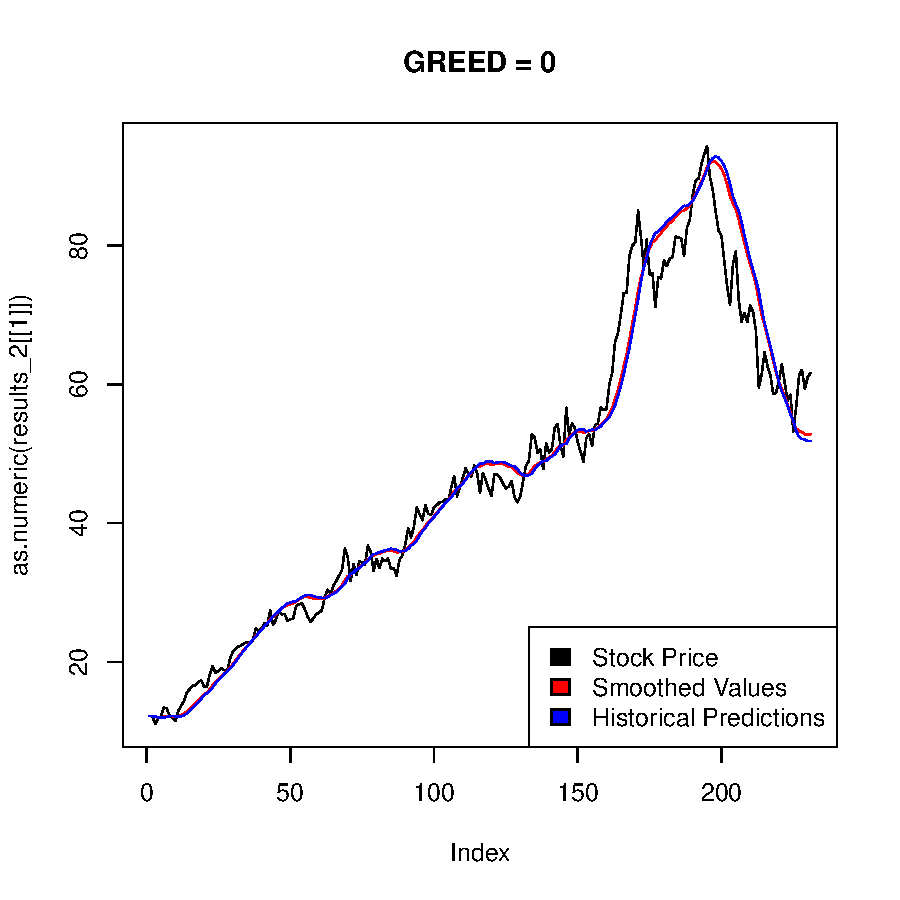
\includegraphics{MV_report-003}

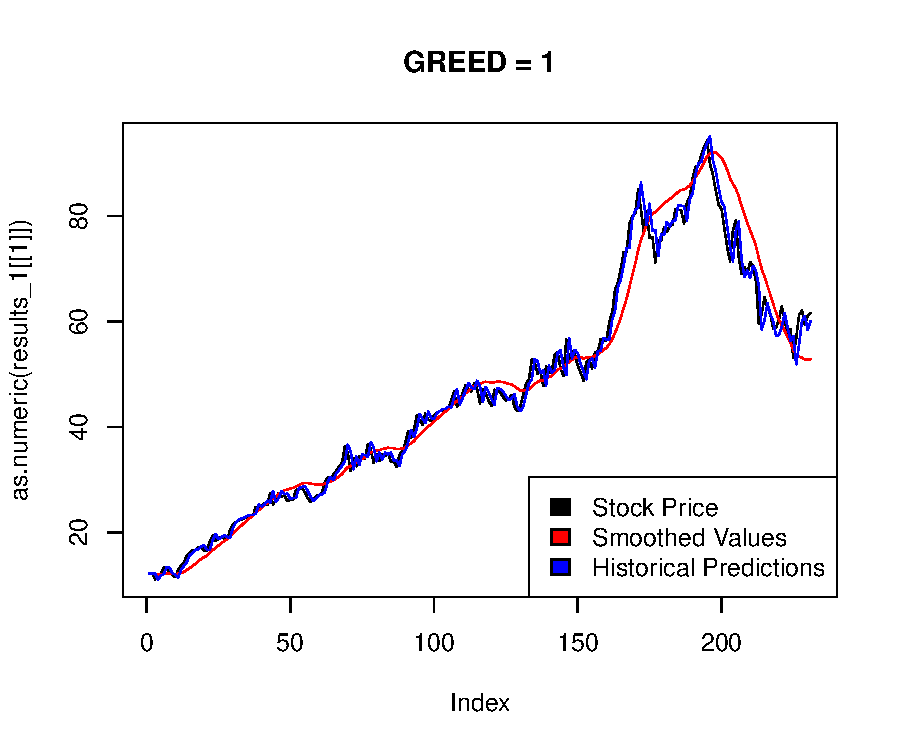
\includegraphics{MV_report-004}

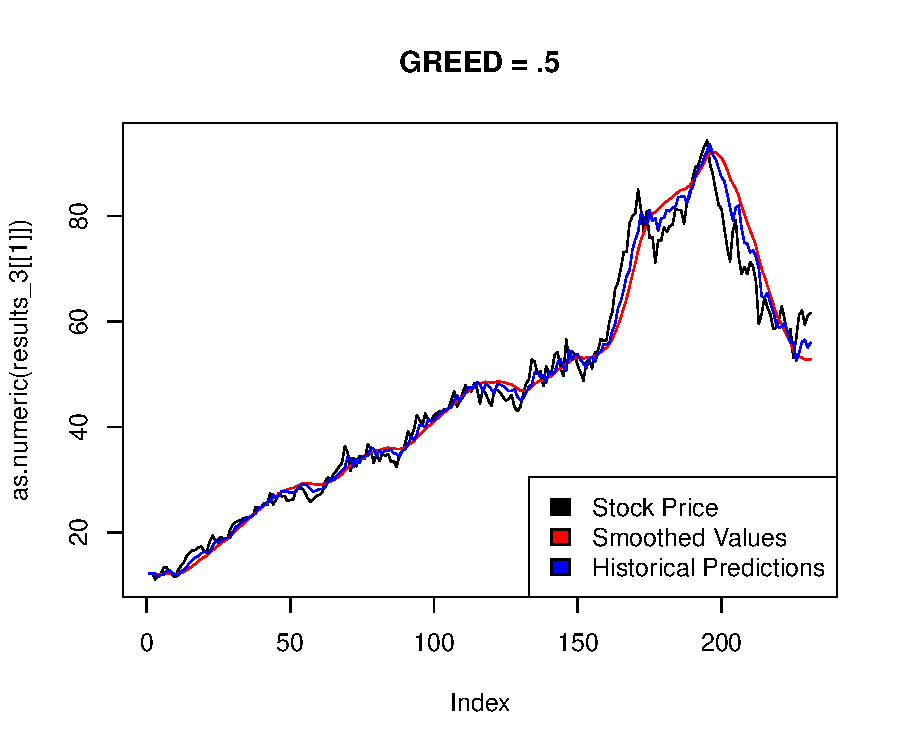
\includegraphics{MV_report-005}

\newpage
\subsection{ Mean Return, Mean Risk, Expected Return}

\section{Results and Comparisons}

\subsection{Two stocks we shall use}

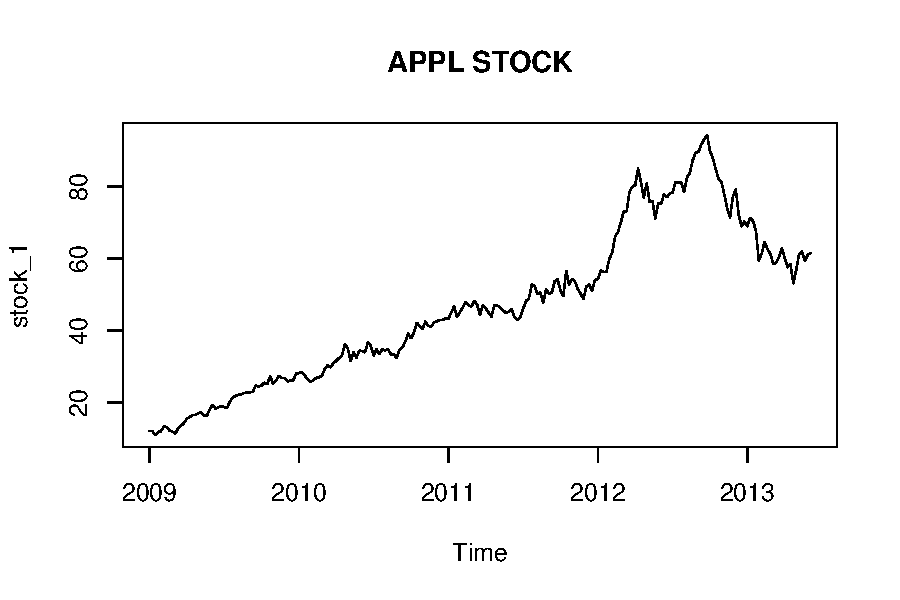
\includegraphics{MV_report-006}

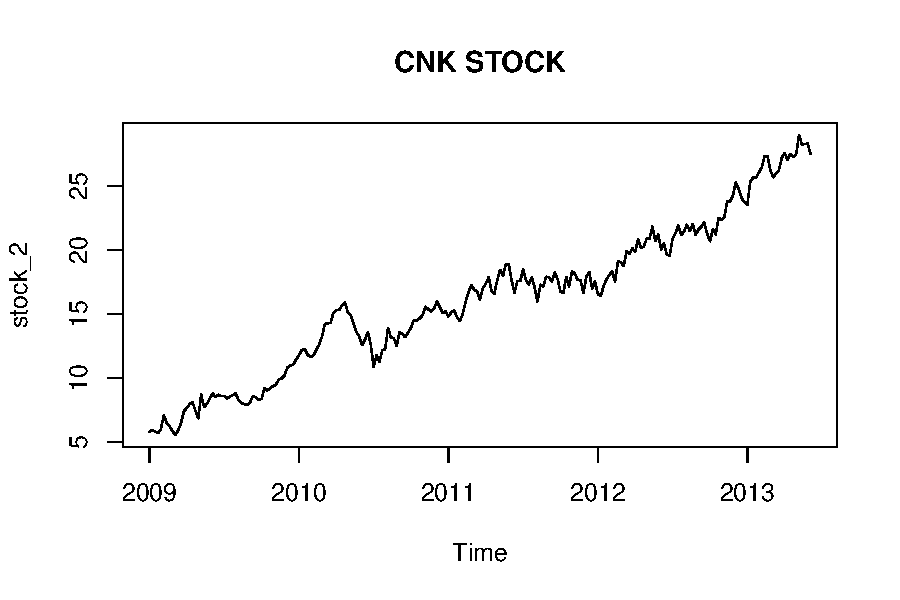
\includegraphics{MV_report-007}
\subsection{Conclusion}

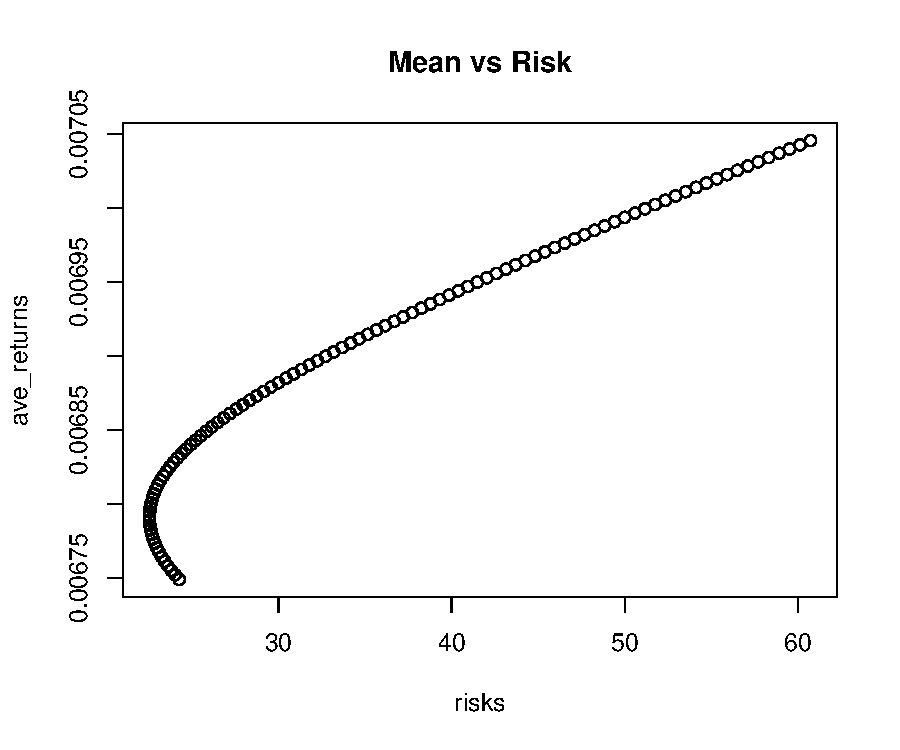
\includegraphics{MV_report-008}

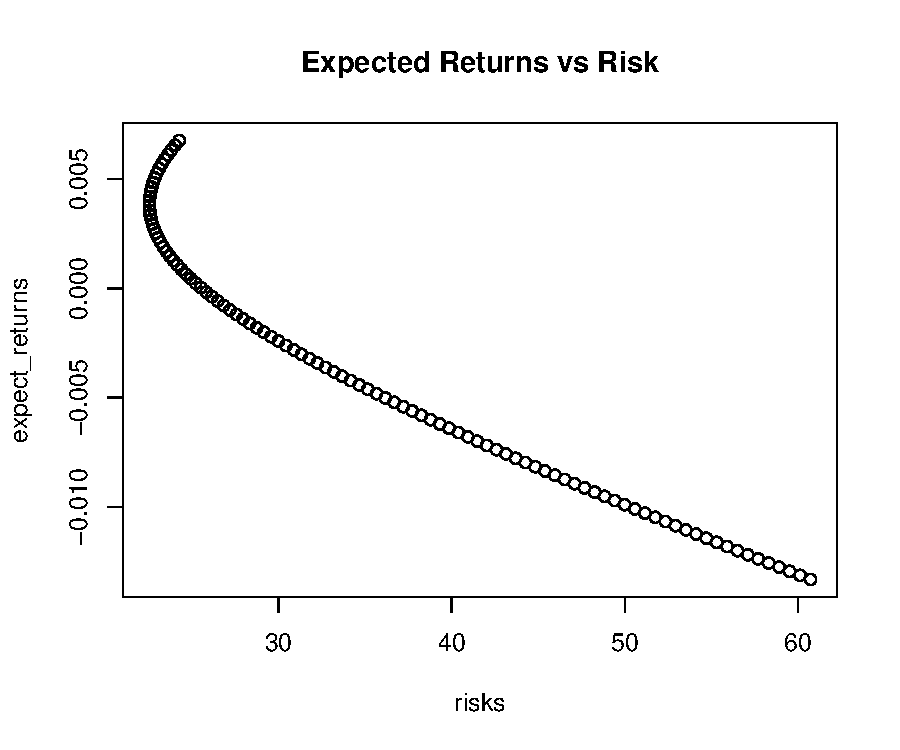
\includegraphics{MV_report-009}

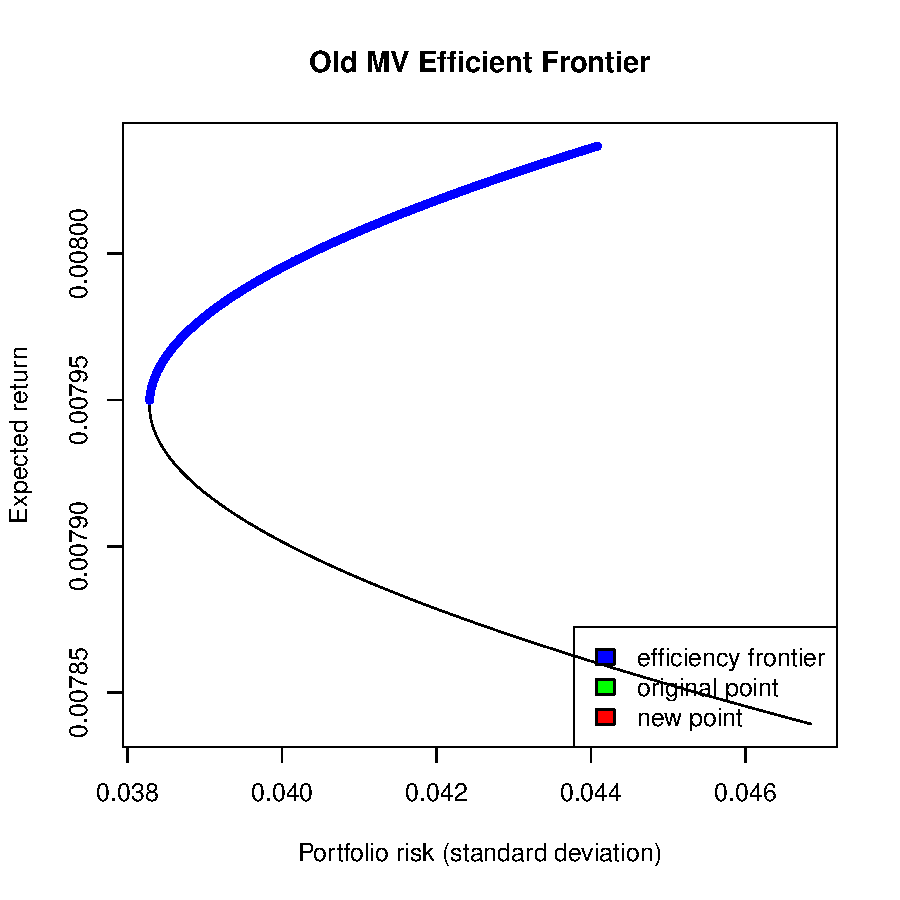
\includegraphics{MV_report-010}

\Large{\indent Above we have three graphs, the first graph is average return plotted against risk. The average return is the amount of return needed to incure every day in order to get the total return rather than mean of all the returns as in the previous MV model. The second graph is the expected return of one time period into the future from our model plotted against the risk. The third graph is the traditional MV Frontier.\\

By comparing the first graph to the third graph, we can see that we have successfully lowered the optimism in the model by not using the averaging returns method. \\
By comparing the second and the third graph we can see that the model recognized that APPL has a current downward trend and CNK has an upward trend. This is why at that point in time the model reccomends to no buy any AAPL because it will neighter decrease the risk of the portfolio nor does it have any predicted returns in the future. Keep in mind that by adjusting alpha, beta, and greed, we will make different predictions. When alpha, beta, and greed are close to zero, we are aiming at making predictions far into the future. When they are close to one, we are making predictions for the near future.}


\end{document}











